\hypertarget{simulation-setup}{%
\chapter{Simulation setup}\label{simulation-setup}}

As stated previously, the core work of this thesis is performing N-body
simulations of the infall of Sgr in the style of Dierickx et
al.~\cite{dierickx_predicted_2017}, varying the initial conditions and dark
matter model to determine the resulting impacts on the evolution of the Sgr
tidal debris stream. As such, we provide an overview of the setup of the
simulations we performed in this section.

\hypertarget{pipeline-and-parameters}{%
\section{Pipeline and parameters}\label{pipeline-and-parameters}}

To begin our experimental pipeline, we first generate the initial
distributions of stellar and dark matter particles using a package called
GalactICS~\cite{deg_galactics_2019}. Each galaxy is modeled using a stellar
disk and dark matter halo. The halo follows a Navarro-Frenk-White (NFW)
profile
\begin{equation}
    \rho_{\text{halo}} (r) = 
    \frac{M_{200}}{4\pi a^3 f(c)} 
    \frac{1}{(r/a)(1+r/a)^2},
\end{equation}
where $f(c) = \log (1+c) - c/(1+c)$, $M_{200}$ is the virial mass, $a$ is the
scale length, $c$ is the concentration, and $c = r_{200} / a$. Here, we use a
lowercase $r$ to denote the radius in a spherical sense.

The stellar disk follows an exponential-sech$^2$ profile, given by
\begin{equation}
    \rho_{\text{disk}} (R, z) = 
    \frac{M_{\text{disk}}}{4 \pi R_0^2 z_0}
    \exp(-R/R_0) \text{ sech}^2(z/z_0),
\end{equation}
where $R_0$ is the disk scale length, $z_0$ is the disk scale height, and the
capital $R$ denotes the cylindrical radius in the plane of the disk.

Both of these distributions are subject to truncation beyond a certain
radius, \(r_t\), with truncation width \(dr_t\). The truncation function
comes from~\cite{widrow_dynamical_2008} and is given by
\begin{equation}
C(r; r_t, dr_t) = \frac{1}{2} \text{erfc} 
\left( \frac{r - r_t}{\sqrt{2} dr_t} \right).
\end{equation}
For the halos, the truncation radius is simply the virial radius and the
truncation width is 20 kpc. For the disks, the truncation radius is 25 kpc,
the width is 5 kpc, and the truncation is only applied to $R$ in the disk
plane. The distributions, including the truncation parameter, can be seen in
Figure~\ref{fig:init_profiles}.

\begin{figure}
    \centering
    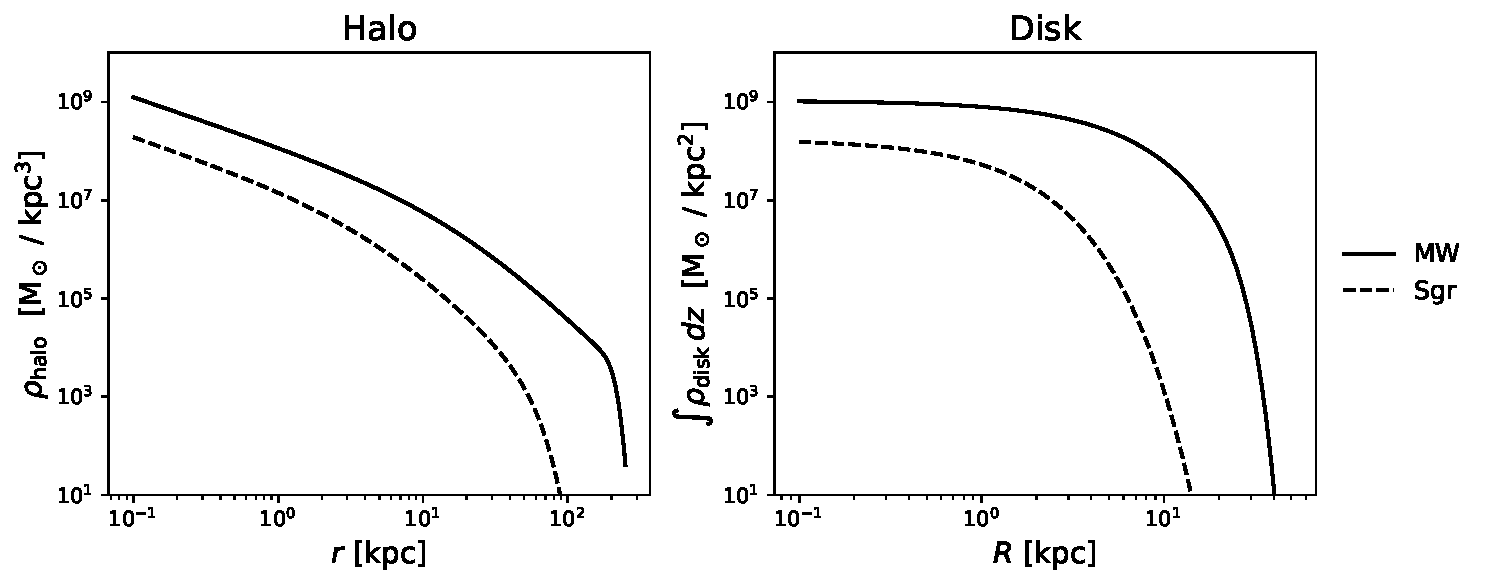
\includegraphics[width=0.9\linewidth]{figs/init_profiles.pdf}
    \caption{%
        Initial profiles for the halo and disk of both galaxies. The halos
        follow a truncated NFW profile and the disks follow a truncated
        exponential-sech$^2$ profile. Note that the disk density is in
        cylindrical coordinates and is integrated over the $z$ direction.
    }
    \label{fig:init_profiles}
\end{figure}

Bundled with GalactICS is a subpackage called GadgetConverters, which
provides a pipeline for converting the native output of GalactICS into a
binary compatible with GADGET and derivative N-body simulation software. In
this work, we use GIZMO~\cite{hopkins_new_2015}, which is itself derived from
GADGET-2~\cite{springel_cosmological_2005}.

\begin{table}
\centering
\begin{tabular}{lcll}
    \toprule
    Parameters & & MW & Sgr \\
    \midrule 
    Halo \\
    $\quad$ Virial mass & $M_{200}$ & $10^{12}$ M$_\odot$ & $10^{10}$ M$_\odot$ \\
    $\quad$ Virial radius & $r_{200}$ & 206 kpc & 44 kpc \\
    $\quad$ Concentration & $c$ & 10 & 8 \\
    $\quad$ Particles & $N_{\text{halo}}$ & $1.16 \times 10^{6}$ & $1.17 \times
    10^{4}$ \\
    Disk \\
    $\quad$ Mass & $M_{\text{disk}}$ & $6.5 \times 10^{10}$ M$_\odot$ & $6 \times 10^{8}$ M$_\odot$ \\
    $\quad$ Scale length & $R_0$ & 3.5 kpc & 0.85 kpc \\
    $\quad$ Scale height & $z_0$ & 0.53 kpc & 0.13 kpc \\
    $\quad$ Particles & $N_{\text{disk}}$ & $2.03 \times 10^{6}$ & $1.17 \times
    10^{4}$ \\
    \bottomrule
\end{tabular}
\caption{%
    Parameters for the initial Milky Way and Sgr galaxies in our full
    simulation. These values are in large part taken from the work
    of~\cite{dierickx_predicted_2017}.
}
\label{tab:sim_params}
\end{table}

The parameters that were used for our simulations were largely taken from the
work of Dierickx et al.~\cite{dierickx_predicted_2017}. They are summarized in
Table~\ref{tab:sim_params}. There are a few key differences between their model
and our simulations, however. First, they used Hernquist profiles for their
halos, while we use NFW distributions. The NFW parameters we use, however, come
from their work, where they are given as the parameters which yield an
approximately equivalent distribution. A comparison between their Hernquist
and our NFW profiles is shown in Figure~\ref{fig:nfw_vs_hernquist}; the
differences are quite small.

\begin{figure}
    \centering
    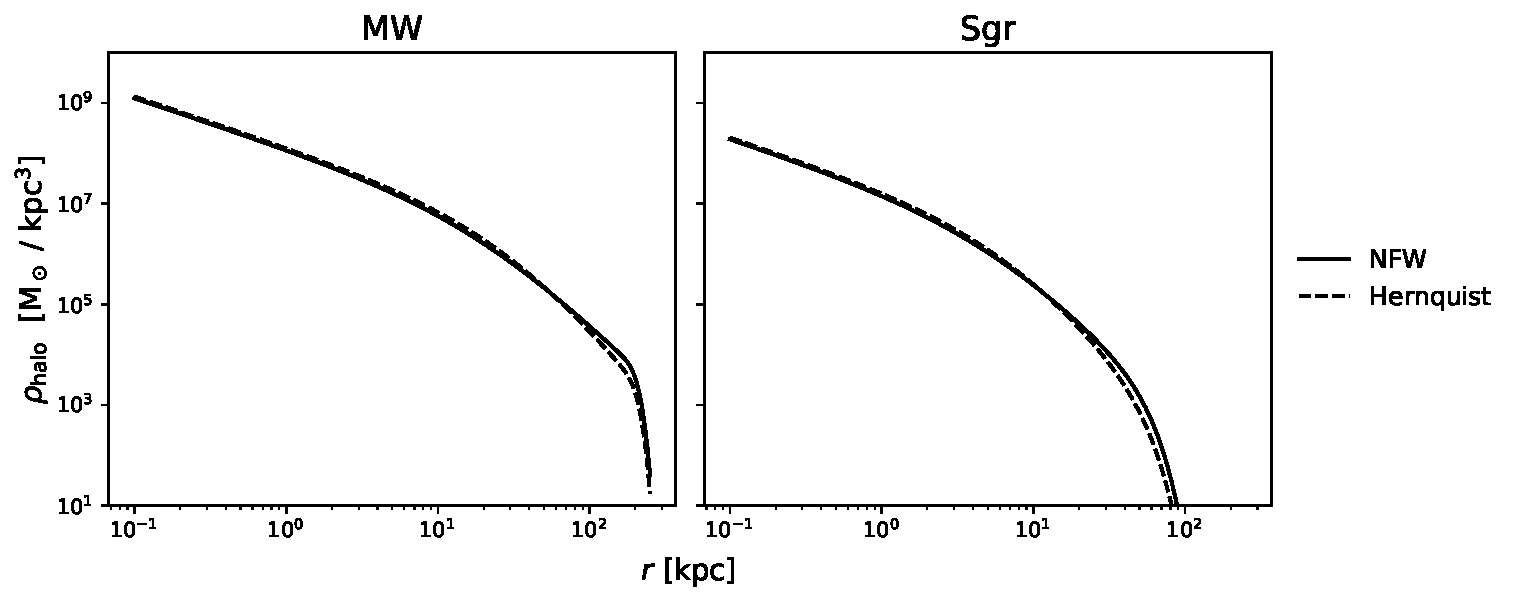
\includegraphics[width=0.9\linewidth]{figs/nfw_vs_hernquist.pdf}
    \caption{%
        Comparison between the density distributions of the relevant truncated
        NFW and truncated Hernquist profiles for the Milky Way and Sgr
        galaxies in the Dierickx model.  The NFW parameters can be found in
        Table~\ref{tab:sim_params}.  The Hernquist parameters are as follows:
        total MW halo mass $1.25 \times 10^{12}$ M$_\odot$, MW scale radius
        $38.35$ kpc, total Sgr halo mass $1.3 \times 10^{10}$ M$_\odot$, Sgr
        scale radius $9.81$ kpc.
    }
    \label{fig:nfw_vs_hernquist}
\end{figure}

The second source of discrepancy between their work and ours is that we have
less resolution in our stellar profile than in their work. This is in part
because they used a Hernquist bulge in both their Milky Way and Sgr, where this
has been omitted from our work. It is also because they used more stellar
particles for the Sgr disk than we did ($1.94 \times 10^4$ versus $1.17 \times
10^4$), owing to a technical error in our initial conditions creation
pipeline.

The experiments performed herein were performed using GIZMO version
2020, built from commit master:0e19830, on Princeton Research Computing's
Della cluster.  This cluster is an Intel cluster with $\geq 20$ cores per node
and $\geq 128$ GB memory per
node~\cite{princeton_research_computing_della_nodate}.  Our simulations often
used around 10 GB of RAM and typically split the computation over 25 cores.

\hypertarget{equilibration}{%
\section{Equilibration}\label{equilibration}}

After generating the initial particle distributions for each galaxy, we
evolved each one forward in time for several Gyrs to allow it to equilibrate.
One reason we do this is because generating initial conditions which are in
equilibrium is a difficult problem, and the initial conditions generator we use
only gives an approximately equilibrated distribution. Evolving it forward in an
isolated system allows the galaxy to come to equilibrium naturally. We have seen
this to be necessary particularly for the Sgr disk distributions.  Another
reason we choose to do this is to create a cored dark matter profile when
using SIDM microphysics.

For each galaxy, we begin with the parameters discussed in the previous
section and perform two equilibration runs: one using CDM microphysics and one
using SIDM microphysics with a velocity independent cross section of \(\sigma
/ m = 10\) cm\(^2\)/g.  In this study, we choose to use a somewhat high cross
section in order to exaggerate any differences that may appear because of the
presence of self-interaction.  We note that future studies should consider a
range of cross sections and velocity dependence.

For the Milky Way equilibrations---both CDM and SIDM---we only evolve the
galaxy forward for 1 Gyr, writing time stamps approximately every 0.1 Gyr.
This is because we expect the initial distribution to be relatively close to
equilibrium, especially when considering such a large galaxy. The resulting
evolution of the mass density profiles are shown in Figure~\ref{fig:mw_evo}.

\begin{figure}
    \centering
    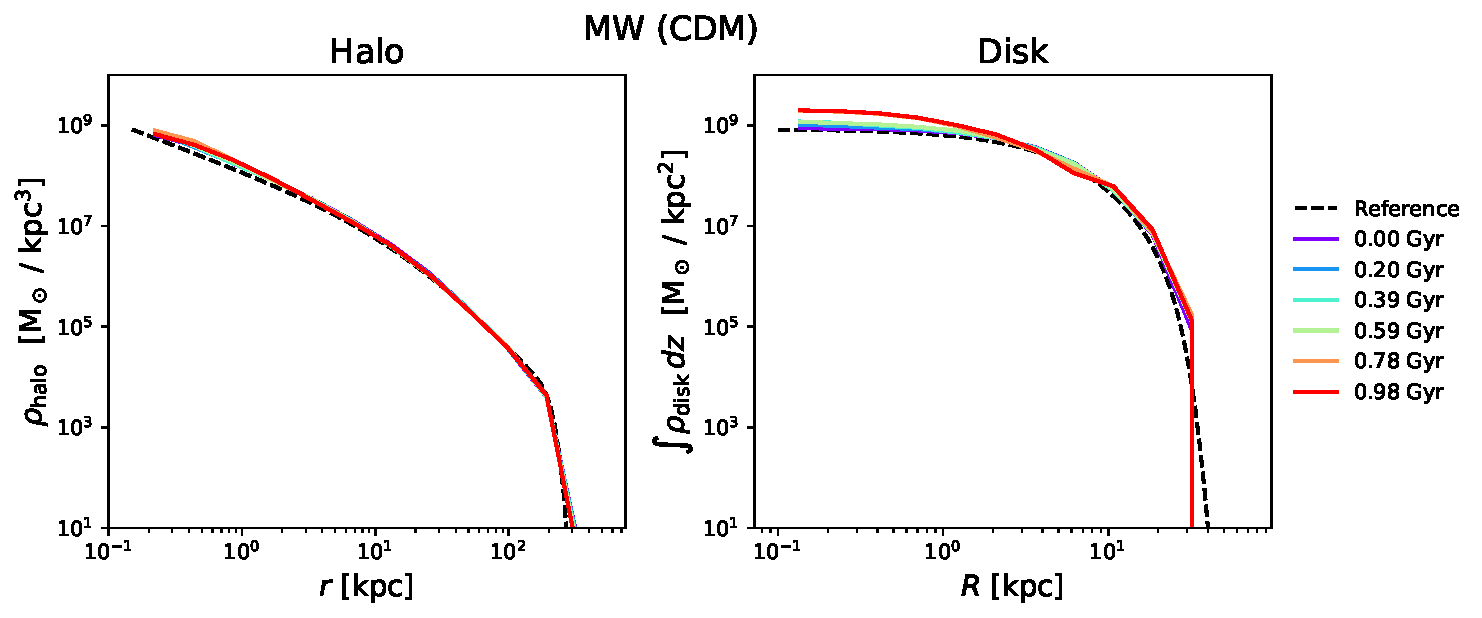
\includegraphics[width=0.9\linewidth]{figs/mw_evolution_cdm.pdf}
    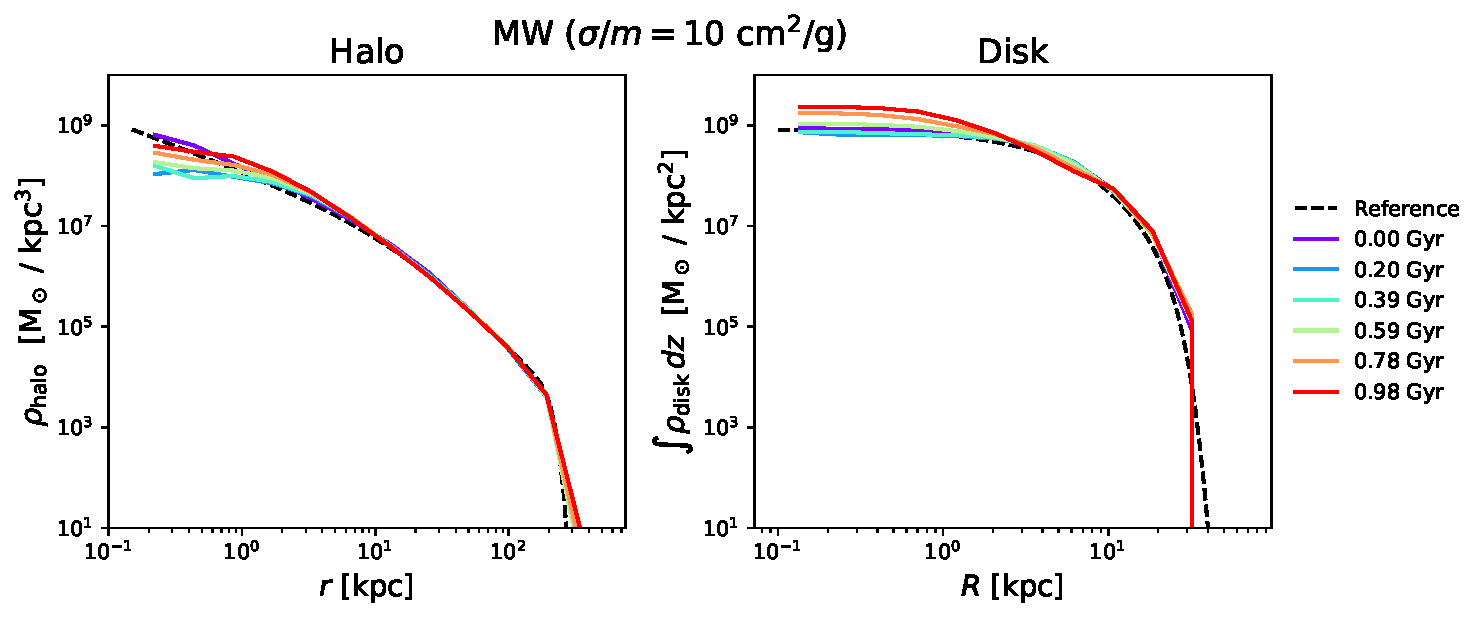
\includegraphics[width=0.9\linewidth]{figs/mw_evolution_sidm.pdf}
    \caption{%
        Evolution of the MW halo (left) and disk (right) during CDM (top) and
        SIDM (bottom) equilibration runs. The dashed line on the halo plots is
        the reference NFW distribution; on the disk plots it is the reference
        exponential-sech$^2$ distribution.
    }
    \label{fig:mw_evo}
\end{figure}

In these plots, we can see that the CDM halo starts in a state which is already
close to equilibrium. The halo changes very little, and the disk slowly pulls
a small amount of density in toward the center. The SIDM halo, however, almost
immedately develops a rather substantial core, which slowly dissolves somewhat,
leaving a small core with size $\sim 1$ kpc. This is almost certainly because
of the disk. As the disk equilibrates, its central density increases,
increasing the gravitational potential in the center of the galaxy and
counteracting the coring effect of self-interactions.

We can also compare these results to those we might have expected following the
analytic formalism for determining the core size in
Section~\ref{analytic-description-with-baryons}. To begin, we need to find the
scale radius $r_0$ and the center value of the gravitational potential
$\Phi_B(0)$ in the ``spherical disk'' approximation. We can do so by using the
following two relations:
\begin{gather}
    \Phi_B(0) = - \frac{G M_B}{r_0} \\
    V_B(r_0) = \frac{\sqrt{-\Phi_B(0)}}{2},
\end{gather}
where $M_B$ is the mass of the baryons in the disk and $V_B$ is the circular
velocity of baryons at the given radius. Together, these imply that $V_B(r_0) =
\sqrt{G M_B / 4 r_0}$.  After truncation, our disk has a total mass of $M_B =
8.1 \times 10^{10}$ M$_\odot$.  Thus, we can plot the rotation curve of our
disk and look for its intersection with $\sqrt{G M_B / 4 r_0}$.  This should
give us the values of $r_0$ and $V_B(r_0)$.  The rotation curves for both the
CDM and SIDM curves are plotted in Figure~\ref{fig:mw_rot_curves}. They show
$r_0 \approx 3.5$ kpc with a corresponding circular velocity $V_B(r_0) \approx
160$ km/s. 

\begin{figure}
    \centering 
    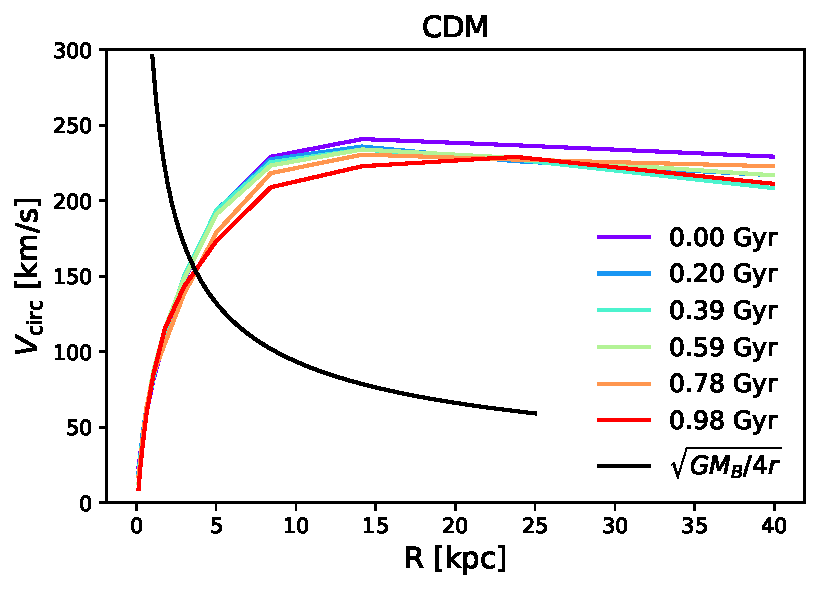
\includegraphics[width=0.45\linewidth]{figs/mw_cdm_rot_curve.pdf}
    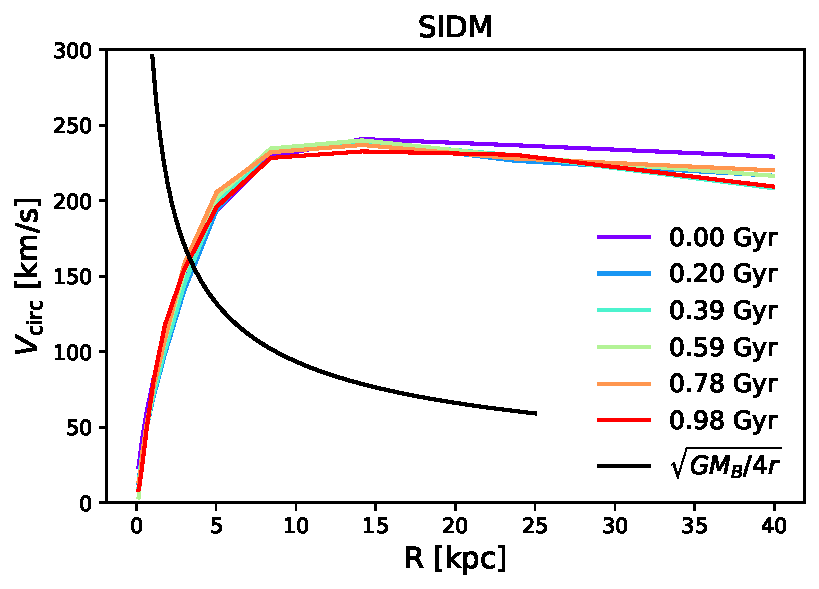
\includegraphics[width=0.45\linewidth]{figs/mw_sidm_rot_curve.pdf}
    \caption{%
        Evolution of rotation curves over time for the Milky Way disk in both
        the CDM and SIDM microphysics runs. Also plotted in black is
        $\sqrt{GM_B/4r}$, the circular velocity at the scale radius which would
        be expected if the disk mass followed a Hernquist profile.
    }
    \label{fig:mw_rot_curves}
\end{figure}

Looking back at Figure~\ref{fig:mw_evo}, we can estimate the central density
of the halo to be $\rho_0 \approx 10^9$ M$_\odot$/kpc$^3$. We can also compute
the central velocity dispersion by finding the root mean square of the radial
velocities for the stars in the inner 5 kpc. For the late CDM snapshots, this
measure gives $\sigma_0 = 123$ km/s.  With all these quantities, we can
compute $a_0 = 43.8$ and $a_1 = 6.6$. Plugging these in to
Equation~\ref{eq:core_size}, we obtain an estimate for the core size of $0.37$
kpc. This core size appears to be roughly consistent with the observed core
size attained in the fully evolved SIDM distribution, though perhaps a little
smaller.

For the Sgr equilibrations, however, we evolved the galaxy much farther
forward in time: approximately 10 Gyr for the CDM case and 20 Gyr for SIDM.
These evolution times do not correspond to a physical orbit (especially given
that the SIDM case would exceed the lifetime of the Universe).  Rather, the
initial Sgr disk distribution was found to be a bit unstable.  We also wanted
to be absolutely certain that the SIDM case would develop a cored profile.
The evolution of the resulting Sgr mass profiles is shown in
Figure~\ref{fig:sgr_evo}.

\begin{figure}
    \centering
    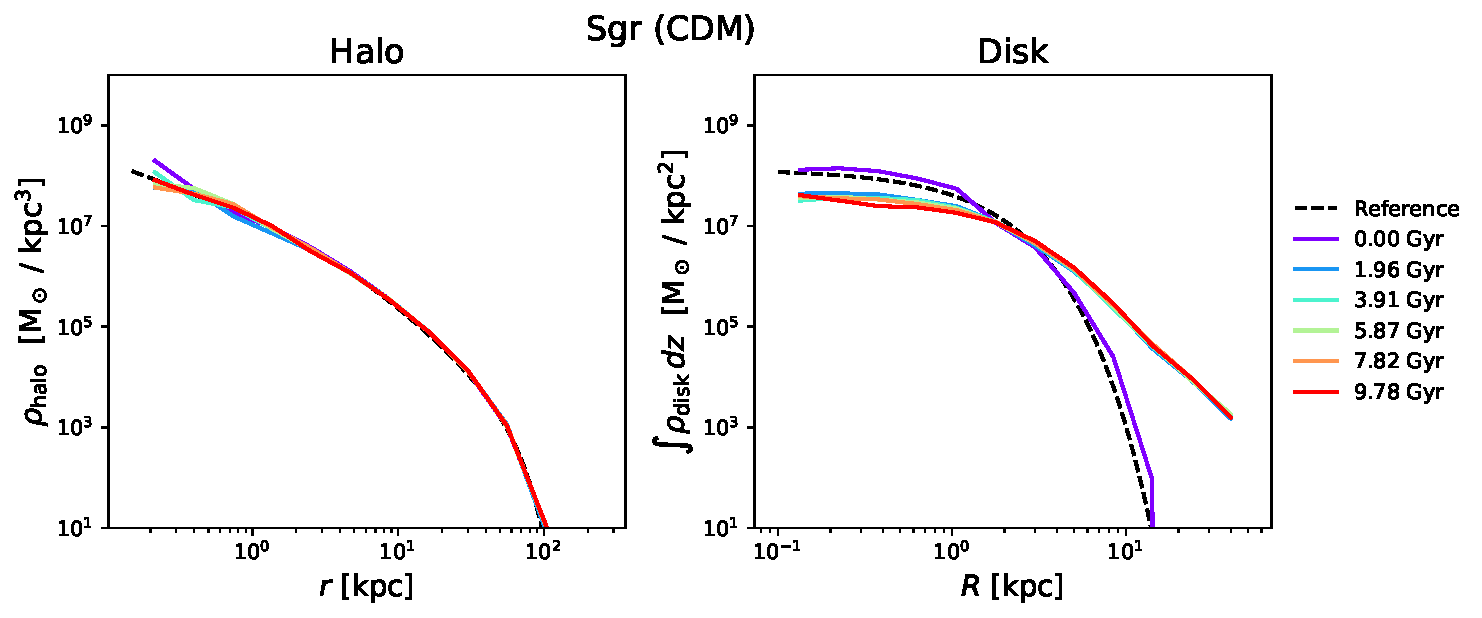
\includegraphics[width=0.9\linewidth]{figs/sgr_evolution_cdm.pdf}
    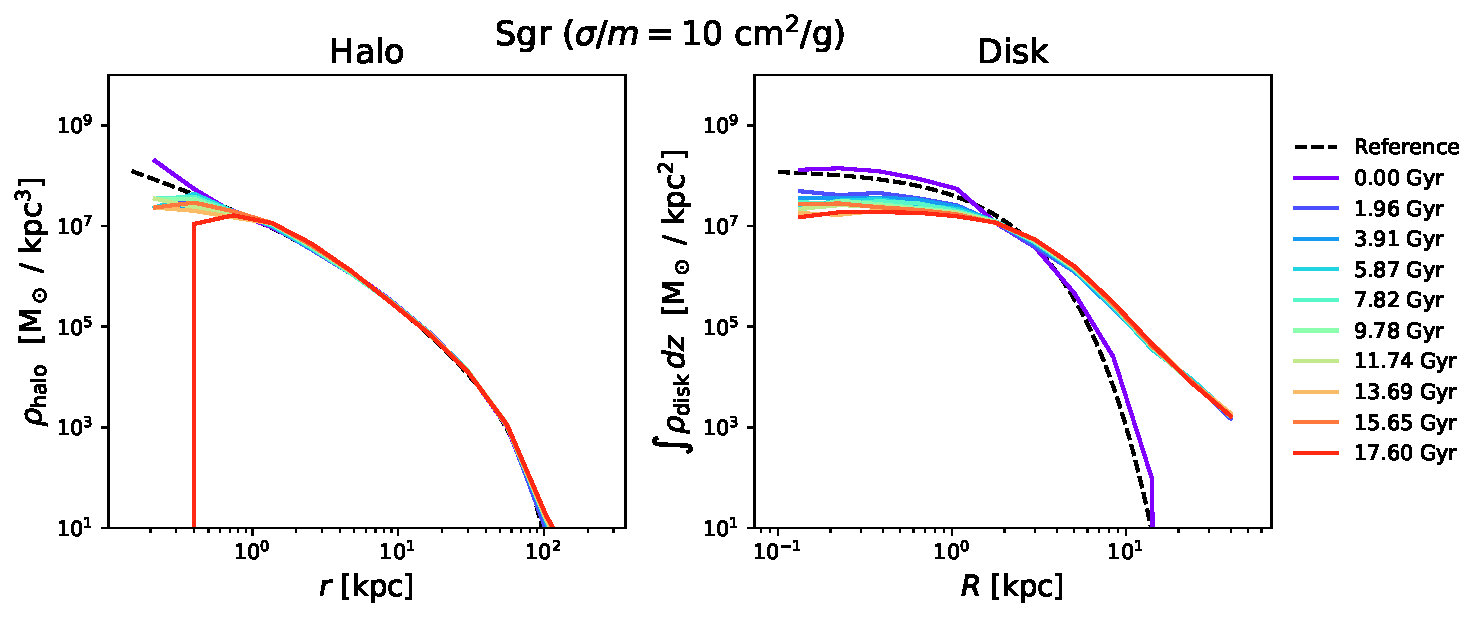
\includegraphics[width=0.9\linewidth]{figs/sgr_evolution_sidm.pdf}
    \caption{%
        Evolution of the Sgr halo (left) and disk (right) during CDM (top) and
        SIDM (bottom) equilibration runs.  The dashed line on the halo plots
        is the reference NFW distribution; on the disk plots it is the
        reference exponential-sech$^2$ distribution.  We note in particular
        that the SIDM run results in generally depressed densities for both
        the halo and disk at low radii.
    }
    \label{fig:sgr_evo}
\end{figure}

In these plots, we see that the initial exponential-sech$^2$ distribution for
the disk was not very close to equilibrium. Almost immediately, the disk
redistributes itself more outwardly, with more of its mass at larger radii and a
falling inner density. In the case of CDM physics, this happens within the first
two Gyr, and the distribution holds relatively constant from there on. In the
SIDM case, however, the distribution appears to continue to adjust, with the
central density falling to around half that of the CDM disk.

In the case of the halo, we notice that the distribution holds relatively
constant in the CDM case and agrees well with the reference NFW distribution. In
the SIDM case, however, we see the slow development of a small core at low
radii. This core appears to have a size of $\approx 1$ kpc. 

We can again apply the analytic expressions derived before to obtain an
estimate for the expected core size.  In this case, we note that the Sgr
galaxy is well-approximated by the dark matter-dominated limit, so we will use
the corresponding limit of the approximate core size.  We again take $r_0 =
3.5$ kpc, and we estimate $\rho_0 \approx 10^{7.5}$ M$_\odot$/kpc$^3$ from
Figure~\ref{fig:sgr_evo}.  We again compute the central velocity dispersion by
finding the root mean square of the radial velocities for the stars in the
inner 5 kpc, which in this case is $\sigma_0 = 26$ km/s.  Using
Equation~\ref{eq:core_dm_dom}, we obtain an estimated core size of $\approx
1.3$ kpc.  We find this to roughly correspond to the core seen in the final
time stamp of the evolved mass density profile.

With the equilibrated MW and Sgr galaxies in both the cuspy and cored régimes,
we combine them to give us two initial conditions for mergers: cuspy and
cored. The Milky Way is left at its position from the equilibration run, as
its center of mass will be close to the origin and its net velocity will be
close to zero. Sgr is placed such that its center of mass lies at the point
\((125, 0, 0)\) kpc and is given an initial velocity \((-10,0,70)\) km/s.
These values correspond to the best fit values found
in~\cite{dierickx_predicted_2017}.
